\documentclass{scrartcl}
\usepackage[T1]{fontenc}
\usepackage[utf8]{inputenc}
\usepackage[ngerman]{babel}
\usepackage{amsmath,amssymb}
\usepackage{graphicx}
\usepackage{enumerate}

\usepackage{tikz}

\definecolor{darkred}{rgb}{0.53,0,.08}

\tikzstyle{rvertex}=[circle,fill=white,minimum size=23pt, inner sep=0pt, text=black, line width=1pt, draw=darkred, font=\Large]
\tikzstyle{bvertex}=[circle,fill=black,minimum size=23pt, inner sep=0pt, text=white, line width=1pt, draw=black, font=\Large]
\tikzstyle{nilvertex}=[rectangle,fill=black,minimum size=12pt, inner sep=0pt, text=white, line width=1pt, draw=black, text width=0.2cm, font=\scriptsize, align=center]
\tikzstyle{niceedge}=[draw, very thick, ->, gray]
\newcommand{\nil}{N\newline I\newline L}

\newcommand{\rbt}{Rot-Schwarz-Baum }


\begin{document}
\section*{Aufgabe 1: Wissensfragen (6 Punkte)}
\begin{enumerate}[(1)]
\item Nennen Sie zwei in der Vorlesung vorgestellte Algorithmen, die nach dem Greedy-Prinzip arbeiten. Begründen Sie kurz, warum. (1P)

\item Nennen Sie einen Vorteil und einen Nachteil von Mergesort gegenüber Quicksort. (1P) 

\item Was bedeutet Stabilität bei Sortieralgorithmen? Nennen Sie eine Situation, in der man die Stabilität ausnutzen kann. (2P)

\item Zeigen oder widerlegen Sie: Bin\"are Suche hat auf jeder Datenstruktur eine bessere Laufzeit als Lineare Suche - Beweisen oder widerlegen sie diese Aussage. (2P)
\end{enumerate}

\section*{Aufgabe 2: Heaps (12 Punkte)}
\begin{enumerate}[(1)]
\item Gegeben sei das folgende Feld: \\
\ \\
\begin{tabular}{|c|c|c|c|c|c|c|c|c|c|c|}
\hline
12 & 21 & 19 & 26 & 99 & 30 & 24 & 32 & 18 & 101 & 128 \\ 
\hline 
\end{tabular} \\
\begin{enumerate}[(a)]
	\item Erläutern Sie, warum das Feld keinen gültigen Min-Heap darstellt. (1P)
	\item Reparieren Sie den Min-Heap mit dem aus der Vorlesung bekannten Verfahren. Geben Sie dabei den Heap nach jeder Änderung an (als Feld oder als Baum). (3P)
\end{enumerate}
\item Gegeben sei ein Datentyp, dessen Elemente bez\"uglich < bzw. > vergleichbar sind. Im folgenden betrachten wir Datenstrukturen f\"ur Elemente dieses Typs.
\begin{enumerate}[(a)]
	\item Warum l\"asst sich in einem Heap das Minimum nicht in $\Theta(1)$ entfernen, sodass die entstehende Struktur immer noch ein Heap ist? (4P) \newline
Hinweis: Betrachten Sie die Laufzeit einer Heapsort-Implementierung, wenn dies möglich wäre. Welcher Widerspruch ergibt sich daraus?

	\item Geben Sie eine Datenstruktur an, die die entsprechende Eigenschaft aus (a) hat. (3P)

	\item Warum ist dies kein Widerspruch zur \"Uberlegung aus (a)? (1P)
\end{enumerate}
\end{enumerate}


\section*{Aufgabe 3: Sortieren (13 Punkte)}
\begin{enumerate}[(1)]
\item Gegebenen sei der Sortieralgorithmus \emph{Cocktail-Sort}. Um ein Array zu sortieren, durchschreitet der Algorithmus den Array zun\"achst von vorne nach hinten und vertauscht dabei zwei benachbarte Werte, wenn sie in der falschen Reihenfolge stehen. Ist der Algorithmus am Ende des Arrays angekommen, durchschreitet er das Array jetzt in umgekehrter Reihenfolge von hinten nach vorne (also \glqq zur\"uck\grqq). Dies wird so lange fortgesetzt, bis in einem Durchlauf keine Elemente mehr vertauscht werden.
\begin{enumerate}[(a)]
\item Wenden Sie Cocktail-Sort auf folgendes Array an, um die Elemente \textbf{aufsteigend} zu sortieren. Geben Sie dabei das Array nach jedem Schritt an. (3P)
\\
\begin{center}
\begin{tabular}{|c|c|c|c|c|c|}
\hline
4 & 2 & 1 & 3 & 7 & 3 \\
\hline
\end{tabular}
\end{center}
\text{ } \\
\item Geben Sie eine naive Implementierung von \emph{Cocktail-Sort} in Pseudocode an. (7P)
\item Geben Sie eine \emph{Familie} von Zahlenarrays an, die von Bubblesort in $O(n^2)$ sortiert werden, aber von Cocktail-Sort in $O(n)$. (3P)
\end{enumerate}
\end{enumerate}

\section*{Aufgabe 4: Dynamische Programmierung (5 Punkte)}
\begin{enumerate}[(1)]

\item Was ist die grundlegende Idee hinter der Methode der dynamischen Programmierung? (1P)

\item Die Fakultätsfunktion $n!$ lässt sich folgendermaßen rekursiv definieren: \newline
$0! = 1$\newline
$n! = n\cdot(n-1)!$ 	für $n \geq 1$
\begin{enumerate}[(a)]
\item Geben Sie ein Programm in Pseudocode an, welches $n!$  mittels dynamischer Programmierung und Bottom-Up-Ansatz berechnet. (3P)
\item Das Programm soll nun so modifiziert werden, dass es nach einmaligem Berechnen von $n!$ jeden Aufruf $k!$ mit $k \leq n$ in $O(1)$ bearbeiten kann. Beschreiben Sie eine Möglichkeit dafür. (1P)
\end{enumerate}
\end{enumerate}

\section*{Aufgabe 5: Datenstrukturen (12 Punkte)}
\begin{enumerate}[(1)]
\item Für die folgenden Anwendungsfälle soll jeweils eine geeignete Datenstruktur ausgewählt werden. Geben Sie jeweils eine passende Datenstruktur an und begründen Sie Ihre Wahl:
\begin{enumerate}[(a)]
\item In einer Musiksammlung sollen häufig neue Musikstücke hinzugefügt, gelöscht und gesucht werden. Über die zukünftige Größe der Sammlung kann beim Anlegen noch keine Aussage gemacht werden. (1P)
\item An einen Datenbankserver werden zu manchen Zeitpunkten so viele Anfragen geschickt, dass er sie nicht sofort bearbeiten kann. Daher soll er die Möglichkeit bekommen, die Anfragen zwischenspeichern zu können, bis er wieder genügend freie Ressourcen besitzt. (1P)
\item Ein Prozess-Scheduler in einem Betriebssystem arbeitet mit unterschiedlich hohen Prioritäten. Bei jedem Aufruf soll jeweils der Prozess mit der höchsten Priorität ausgeführt werden, wobei die Auswahlgeschwindigkeit für die Leistungsfähigkeit des Betriebssystems eine entscheidende Rolle spielt. (1P)
\end{enumerate}

\item Zeigen Sie, wie eine Warteschlange mit einer \textbf{einfach verketteten} Liste sowie zwei Zeigern \textit{K} (ältestes Element) und \textit{E} (neuestes Element) implementiert werden kann. Hierbei sollen sowohl ENQUEUE(X) als auch DEQUEUE() die Laufzeit O(1) besitzen. (4P)\\
Gehen Sie dafür folgendermaßen vor:\\
\begin{itemize}
	\item Stellen Sie mit einer Skizze dar, wie die beiden Zeiger in der Liste positioniert werden müssen.
	\item Geben Sie den Pseudocode für beide Warteschlangenoperationen an. Stellen  Sie dabei sicher, dass Ihre Implementierung auch korrekt mit einer leeren Warteschlange umgehen kann.
\end{itemize}

\item Löschen Sie in folgendem Rot-Schwarz-Baum die 17 und zeichenen Sie den reparierten Baum. (5P)

\begin{center}
\begin{tikzpicture}[level 1/.style={level distance = 1.2cm}, level 2/.style={sibling distance=50mm}, level 3/.style={sibling distance=30mm}, level 4/.style={sibling distance=12mm}, scale=1, level 5/.style={sibling distance=6mm}, scale=1]
   \node {}
    child {node [bvertex] {13} edge from parent[niceedge]
     child {node [rvertex] {8}
      child {node [bvertex]  {1}
      	child {node [nilvertex] {\nil}}
      	child {node [rvertex] {6}
	 child {node [nilvertex] {\nil}}
      	 child {node [nilvertex] {\nil}}
	}
      }
      child {node [bvertex]  {11}
      	child {node [nilvertex] {\nil}}
      	child {node [nilvertex] {\nil}}
      } 
    }
    child {node [rvertex] {17}
     child {node [bvertex] {15}
      child {node [nilvertex] {\nil}}
      child {node [nilvertex] {\nil}}
     }
     child {node [bvertex] {25}
      child {node [rvertex] {22}
       child {node [nilvertex] {\nil}}
       child {node [nilvertex] {\nil}}
      }
      child {node [rvertex] {27}
       child {node [nilvertex] {\nil}}
       child {node [nilvertex] {\nil}}
      }
     }
    }
   };
\end{tikzpicture}
\end{center}

\end{enumerate}

\section*{Aufgabe 6: Graphen (12 Punkte)}
\begin{enumerate}[(1)]
\item Ein Graph G = (V,E) sei durch die folgende Adjazenzfelddarstellung gegeben:\\
\ \\
V := \begin{tabular}{|c|c|c|c|c|c|}
\hline 
1 & 3 & 4 & 6 & 9 & 11 \\ 
\hline 
\end{tabular}  \\
\ \\
E := \begin{tabular}{|c|c|c|c|c|c|c|c|c|c|c|}
\hline 
2 & 3 & 4 & 2 & 5 & 2 & 3 & 6 & 1 & 6 & 5 \\ 
\hline 
\end{tabular}\\
\begin{enumerate}[(a)]
	\item Zeichnen Sie den Graphen. (2P)
	\item Geben Sie den Graphen in Adjazenzlistendarstellung an. (1P)
	\item Welche dritte Möglichkeit zur Darstellung von Graphen wurde in der Vorlesung vorgestellt? Beschreiben Sie sie kurz und nennen Sie sowohl einen Vor- als auch einen Nachteil dieser Methode. (2P)
\end{enumerate} 

\item Wenden Sie den Algorithmus von Prim auf dem folgenden Graphen an. Der Startknoten sei a. Markieren Sie die Kanten des resultierenden MSTs eindeutig (z.B. durch dicke Linien) und geben Sie die Reihenfolge der hinzugefügten Kanten an. (2P)
\begin{figure}[h]
\centering
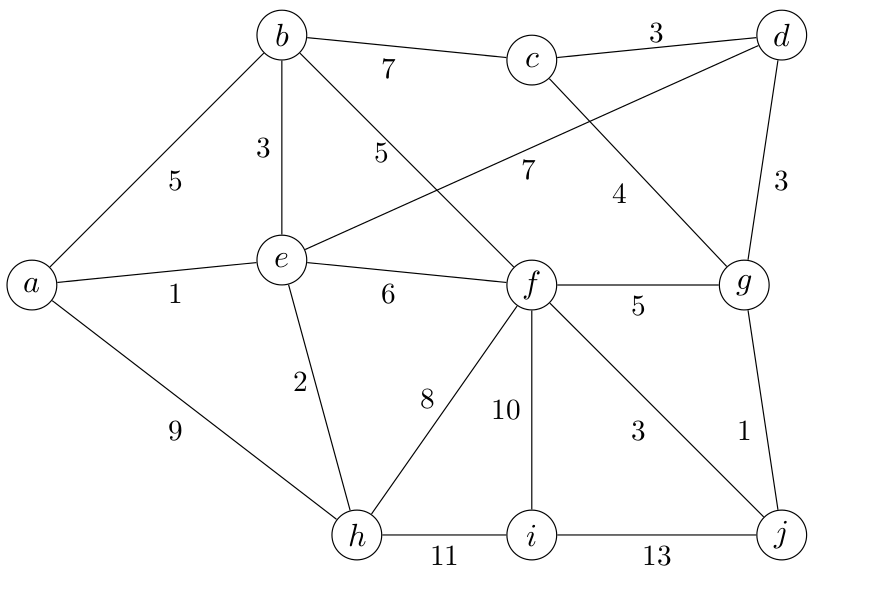
\includegraphics[width=0.66\textwidth]{mst_graph.png}
\end{figure}

\item Gegeben sei folgender Graph:\\
\ \\
\begin{center}
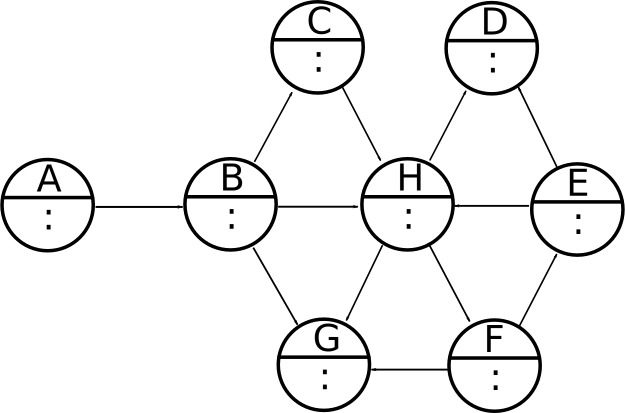
\includegraphics[width=0.75\linewidth]{images/tiefensuche_aufg}\\
\end{center}
Führen Sie auf diesem Graphen eine Tiefensuche aus und gehen Sie dabei wie folgt vor:
\begin{itemize}
	\item Beginnen Sie bei Knoten A.
	\item Die Betrachtung der ausgehenden Kanten eines Knotens soll im Uhrzeigersinn erfolgen
	\item Schreiben Sie die \textit{discovered}-Zeiten der Knoten links neben die Doppelpunkte, die \textit{finalized}-Zeiten jeweils rechts daneben.
	\item Klassifzieren Sie die Kanten:
	\begin{itemize}
		\item jede \textit{Baumkante} durch eine dicke Linie
		\item jede \textit{Rückwärtskante} mit einem ''B''
		\item jede \textit{Vorwärtskante} mit einem ''F''
		\item jede \textit{Querkante} mit einem ''C''
	\end{itemize} 
\end{itemize}
(5P)
\end{enumerate}
\end{document}